\documentclass[portrait,final,a1paper,fontscale=0.401]{baposter}

\usepackage{calc}
\usepackage{graphicx}
\usepackage{amsmath}
\usepackage{amssymb}
\usepackage{relsize}
\usepackage{multirow}
\usepackage{rotating}
\usepackage{bm}
\usepackage{url}

\usepackage{setspace}

\usepackage{graphicx}
\usepackage{multicol}

%\usepackage{times}
%\usepackage{helvet}
%\usepackage{bookman}
\usepackage{palatino}

\newcommand{\captionfont}{\footnotesize}

\graphicspath{{images/}{../images/}}
\usetikzlibrary{calc}

\newcommand{\SET}[1]  {\ensuremath{\mathcal{#1}}}
\newcommand{\MAT}[1]  {\ensuremath{\boldsymbol{#1}}}
\newcommand{\VEC}[1]  {\ensuremath{\boldsymbol{#1}}}
\newcommand{\Video}{\SET{V}}
\newcommand{\video}{\VEC{f}}
\newcommand{\track}{x}
\newcommand{\Track}{\SET T}
\newcommand{\LMs}{\SET L}
\newcommand{\lm}{l}
\newcommand{\PosE}{\SET P}
\newcommand{\posE}{\VEC p}
\newcommand{\negE}{\VEC n}
\newcommand{\NegE}{\SET N}
\newcommand{\Occluded}{\SET O}
\newcommand{\occluded}{o}

%%%%%%%%%%%%%%%%%%%%%%%%%%%%%%%%%%%%%%%%%%%%%%%%%%%%%%%%%%%%%%%%%%%%%%%%%%%%%%%%
%%%% Some math symbols used in the text
%%%%%%%%%%%%%%%%%%%%%%%%%%%%%%%%%%%%%%%%%%%%%%%%%%%%%%%%%%%%%%%%%%%%%%%%%%%%%%%%

%%%%%%%%%%%%%%%%%%%%%%%%%%%%%%%%%%%%%%%%%%%%%%%%%%%%%%%%%%%%%%%%%%%%%%%%%%%%%%%%
% Multicol Settings
%%%%%%%%%%%%%%%%%%%%%%%%%%%%%%%%%%%%%%%%%%%%%%%%%%%%%%%%%%%%%%%%%%%%%%%%%%%%%%%%
\setlength{\columnsep}{1.5em}
\setlength{\columnseprule}{0mm}

%%%%%%%%%%%%%%%%%%%%%%%%%%%%%%%%%%%%%%%%%%%%%%%%%%%%%%%%%%%%%%%%%%%%%%%%%%%%%%%%
% Save space in lists. Use this after the opening of the list
%%%%%%%%%%%%%%%%%%%%%%%%%%%%%%%%%%%%%%%%%%%%%%%%%%%%%%%%%%%%%%%%%%%%%%%%%%%%%%%%
\newcommand{\compresslist}{%
\setlength{\itemsep}{1pt}%
\setlength{\parskip}{0pt}%
\setlength{\parsep}{0pt}%
}

%%%%%%%%%%%%%%%%%%%%%%%%%%%%%%%%%%%%%%%%%%%%%%%%%%%%%%%%%%%%%%%%%%%%%%%%%%%%%%
%%% Begin of Document
%%%%%%%%%%%%%%%%%%%%%%%%%%%%%%%%%%%%%%%%%%%%%%%%%%%%%%%%%%%%%%%%%%%%%%%%%%%%%%

\begin{document}

%%%%%%%%%%%%%%%%%%%%%%%%%%%%%%%%%%%%%%%%%%%%%%%%%%%%%%%%%%%%%%%%%%%%%%%%%%%%%%
%%% Here starts the poster
%%%---------------------------------------------------------------------------
%%% Format it to your taste with the options
%%%%%%%%%%%%%%%%%%%%%%%%%%%%%%%%%%%%%%%%%%%%%%%%%%%%%%%%%%%%%%%%%%%%%%%%%%%%%%
% Define some colors

%\definecolor{lightblue}{cmyk}{0.83,0.24,0,0.12}
\definecolor{lightblue}{rgb}{0.5,0.8,1}
\definecolor{darkblue}{rgb}{0.5,0.8,1}
\definecolor{myblue}{rgb}{0.2,0.7,0.2}

% Draw a video
\newlength{\FSZ}
\newcommand{\drawvideo}[3]{% [0 0.25 0.5 0.75 1 1.25 1.5]
   \noindent\pgfmathsetlength{\FSZ}{\linewidth/#2}
   \begin{tikzpicture}[outer sep=0pt,inner sep=0pt,x=\FSZ,y=\FSZ]
   \draw[color=lightblue!50!black] (0,0) node[outer sep=0pt,inner sep=0pt,text width=\linewidth,minimum height=0] (video) {\noindent#3};
   \path [fill=lightblue!50!black,line width=0pt] 
     (video.north west) rectangle ([yshift=\FSZ] video.north east) 
    \foreach \x in {1,2,...,#2} {
      {[rounded corners=0.6] ($(video.north west)+(-0.7,0.8)+(\x,0)$) rectangle +(0.4,-0.6)}
    }
;
   \path [fill=lightblue!50!black,line width=0pt] 
     ([yshift=-1\FSZ] video.south west) rectangle (video.south east) 
    \foreach \x in {1,2,...,#2} {
      {[rounded corners=0.6] ($(video.south west)+(-0.7,-0.2)+(\x,0)$) rectangle +(0.4,-0.6)}
    }
;
   \foreach \x in {1,...,#1} {
     \draw[color=lightblue!50!black] ([xshift=\x\linewidth/#1] video.north west) -- ([xshift=\x\linewidth/#1] video.south west);
   }
   \foreach \x in {0,#1} {
     \draw[color=lightblue!50!black] ([xshift=\x\linewidth/#1,yshift=1\FSZ] video.north west) -- ([xshift=\x\linewidth/#1,yshift=-1\FSZ] video.south west);
   }
   \end{tikzpicture}
}

\hyphenation{resolution occlusions}
%%
\begin{poster}%
  % Poster Options
  {
  % Show grid to help with alignment
  grid=false,
  % Column spacing
  colspacing=1em,
  % Color style
  bgColorOne=white,
  bgColorTwo=white,
  borderColor=lightblue,
  headerColorOne=darkblue,
  headerColorTwo=lightblue,
  headerFontColor=black,
  boxColorOne=white,
  boxColorTwo=lightblue,
  % Format of textbox
  textborder=roundedleft,
  % Format of text header
  eyecatcher=true,
  headerborder=closed,
  headerheight=0.1\textheight,
%  textfont=\sc, An example of changing the text font
  headershape=roundedright,
  headershade=shadelr,
  headerfont=\Large\bf\textsc, %Sans Serif
  textfont={\setlength{\parindent}{0.5em}},
  boxshade=plain,
%  background=shade-tb,
  background=plain,
  linewidth=2pt
  }
  % Eye Catcher
  {} 
  % Title
  {\bf\textsc{Additive regularization of topic model: \\ Convergence results}\vspace{0.5em}}
  % Authors
  {\textsc{Ilya Irkhin, ilirhin@gmail.com }}
  % University logo
  {% The makebox allows the title to flow into the logo, this is a hack because of the L shaped logo.
    %\includegraphics[height=9.0em]{images/msu.png}
  }

%%%%%%%%%%%%%%%%%%%%%%%%%%%%%%%%%%%%%%%%%%%%%%%%%%%%%%%%%%%%%%%%%%%%%%%%%%%%%%
%%% Now define the boxes that make up the poster
%%%---------------------------------------------------------------------------
%%% Each box has a name and can be placed absolutely or relatively.
%%% The only inconvenience is that you can only specify a relative position 
%%% towards an already declared box. So if you have a box attached to the 
%%% bottom, one to the top and a third one which should be in between, you 
%%% have to specify the top and bottom boxes before you specify the middle 
%%% box.
%%%%%%%%%%%%%%%%%%%%%%%%%%%%%%%%%%%%%%%%%%%%%%%%%%%%%%%%%%%%%%%%%%%%%%%%%%%%%%
    %
    
    % A coloured circle useful as a bullet with an adjustably strong filling
    \newcommand{\colouredcircle}{%
      \tikz{\useasboundingbox (-0.2em,-0.32em) rectangle(0.2em,0.32em); \draw[draw=headerColorOne,fill=lightblue,line width=0.03em] (0,0) circle(0.18em);}}


%%%%%%%%%%%%%%%%%%%%%%%%%%%%%%%%%%%%%%%%%%%%%%%%%%%%%%%%%%%%%%%%%%%%%%%%%%%%%%
  \headerbox{Topic modeling}{name=artm,column=0, span=1}{
%%%%%%%%%%%%%%%%%%%%%%%%%%%%%%%%%%%%%%%%%%%%%%%%%%%%%%%%%%%%%%%%%%%%%%%%%%%%%%
	\textbf{Given:}
	
	$ D $ is a set of documents, $ W $ is a set of terms, $n_{dw}$ is a frequency of term $w$ in document $d$. %Denote $F_{dw} =  p(w|d)  = \frac{n_{dw}}{n_d}$
	
	\medskip\textbf{Find} model: 
	\[ 
	p(w|d) = \sum_{t\in T} p(w|t) p(t|d) = \sum_{t\in T} \varphi_{wt} \theta_{td}
	\] 
	with parameters $\varphi_{wt}$, $\theta_{td}$:
	%$ \Phi = (\varphi_{wt})_{W \times T}$, 
	%$ \Theta = (\theta_{td})_{T \times D} $:
	\begin{itemize}
	\item $ \varphi_{wt} = p(w|t) $ is a distribution over terms in topic $ t $;
	\item $ \theta_{td} = p(t|d) $ is a distribution over topics in document $ d $. 
	\end{itemize}
	
	\textbf{Optimization task} is
	regularized likelihood maximization:
  \[\small
        \underbrace{\sum_{d\in D} \sum_{w\in d} \!n_{dw} \ln \sum_{t\in T} \phi_{wt}\theta_{td}}_{L(\Phi,\Theta)}
        +
        {\underbrace{{\sum_{i=1}^n \tau_i R_i(\Phi,\Theta)}}_{R(\Phi,\Theta)}}
        \to \max _{\Phi,\Theta}
   \]
	 where $R(\Phi, \Theta)$ is a weighted sum of regularization criteria.
  }


%Here could be Contributions 

%%%%%%%%%%%%%%%%%%%%%%%%%%%%%%%%%%%%%%%%%%%%%%%%%%%%%%%%%%%%%%%%%%%%%%%%%%%%%%
\headerbox{Regularized EM}{name=baseem, column=1, row=0}{
    Applying Karush--Kuhn--Tucker theorem, 
    one can obtain the following EM-algorithm:
    
   \textbf{E-step:}
    
    $p_{tdw} \propto \varphi_{wt} \theta_{td}$
 \smallskip
   
    \textbf{M-step:}
    
    $n_{wt} = \sum\limits_{d \in D} n_{dw} p_{tdw}$
    
    $n_{td} = \sum\limits_{w \in W} n_{dw} p_{tdw}$
    
   $r_{wt} =  \phi_{wt}\tfrac{\partial R}{\partial\phi_{wt}}$, $r_{td} =  \theta_{td}\tfrac{\partial R}{\partial\theta_{td}}$

    $\phi_{wt}   \propto \bigl(n_{wt} + r_{wt} \bigr)_{\!+}$, $\theta_{td} \propto  \bigl(n_{td} + r_{td}\bigr)_{\!+}$
}


%%%%%%%%%%%%%%%%%%%%%%%%%%%%%%%%%%%%%%%%%%%%%%%%%%%%%%%%%%%%%%%%%%%%%%%%%%%%%%
  \headerbox{Unbiased Modification}{name=em,column=2,row=0}{
%%%%%%%%%%%%%%%%%%%%%%%%%%%%%%%%%%%%%%%%%%%%%%%%%%%%%%%%%%%%%%%%%%%%%%%%%%%%%%
    Replacing $\phi_{wt}$ and $\theta_{td}$ with their unbiased maximum likelihood estimators on M-step doesn't deteriorate the convergence but simplifies calculations:
    
  $ r_{wt} =  \frac{n_{wt}}{n_t}\dfrac{\partial R}{\partial\phi_{wt}} \big( \frac{n_{wt}}{n_t},  \frac{n_{td}}{n_d} \big)$

   $r_{td} =\frac{n_{td}}{n_d}\dfrac{\partial R}{\partial\theta_{td}}  \big( \frac{n_{wt}}{n_t},  \frac{n_{td}}{n_d} \big)$
    
    \vspace{0.8em}
    Under conditions of the convergence theorem and with this modification  one can estimate the change of $R$ on M-step:
\[
\Delta R=  \frac12 \sum\limits_{t, w, u}   \frac{1}{\sum\limits_v n_{vt}} \bigg(  \frac{\partial{R}}{\partial{\phi_{wt}}}  -  \frac{\partial{R}}{\partial{\phi_{ut}}}  \bigg)^2 \phi_{wt} \phi_{ut}  + 
\]
\[
+ \frac12 \sum\limits_{d, t, s}   \frac{1}{\sum\limits_r n_{rd}} \bigg(  \frac{\partial{R}}{\partial{\theta_{td}}}  -  \frac{\partial{R}}{\partial{\theta_{sd}}}  \bigg)^2 \theta_{td} \theta_{sd}  \geq 0
\]
}



  \headerbox{Convergence theorem}{name=convergence,column=1,below=baseem}{
Denote $x^k$ as value of $x$ on $k$-th iteration.
 Suppose that
\begin{enumerate}
\item  $ n^k_{wt} = 0 \Rightarrow \phi^k_{wt} = 0$ , $n^k_{td} = 0 \Rightarrow \theta^k_{td} = 0$ -- saving zero.
\item $\exists \varepsilon>0\ \exists N\ \forall k > N\ \phi^k_{wt}, \theta^k_{td} \notin (0, \varepsilon)$ -- separability from zero.
\item  $ n_{dw}>0 \Rightarrow \forall k\ \exists t\colon p^k_{tdw} > 0$ -- likelihood is finite during iterations.
\item $\exists \delta >0\ \exists N\ \forall k > N \ \forall t\ \exists w\  n^k_{wt} + r^k_{wt} > \delta$ and the similar condition for $\theta$ -- separability from zero of the denominator. It's a criteria for topic selection.
\item $\exists N\ \forall k > N\colon\ \ Q^k (\phi^k, \theta^k)+ R(\phi^k, \theta^k) \geq Q^k(\phi^{k-1}, \theta^{k-1}) + R(\phi^{k-1}, \theta^{k-1})$, where $Q^k(\phi, \theta) = \sum\limits_{t,d,w} p^k_{tdw} (\ln \phi_{wt} + \ln \theta_{td})$ -- Increase of the lower bound of regularized likelihood during iterations. 
\end{enumerate}
Then for  $k \to \infty$
\[
\|\phi^k - \phi^{k-1}\|_1 \to 0, \|\theta^k - \theta^{k-1}\|_1 \to 0 .
\]
  }
%%%%%%%%%%%%%%%%%%%%%%%%%%%%%%%%%%%%%%%%%%%%%%%%%%%%%%%%%%%%%%%%%%%%%%%%%%%%%%

  \headerbox{Gradient Modification}{name=eme,column=2,below=em}{
%%%%%%%%%%%%%%%%%%%%%%%%%%%%%%%%%%%%%%%%%%%%%%%%%%%%%%%%%%%%%%%%%%%%%%%%%%%%%%
One suggests to use the gradient of regulariser as regularization additives. It may improve the convergence and doesn't complicate the calculations.
\smallskip
\smallskip

$r_{wt} =  \frac{1}{\sum\limits_w n_{wt}} \big( \frac{\partial{R}}{\partial{\phi_{wt}}} - \sum\limits_u \phi_{ut} \frac{\partial{R}}{\partial{\phi_{ut}}} \big)$

$ r_{td} =  \frac{1}{\sum\limits_t n_{td}} \big( \frac{\partial{R}}{\partial{\theta_{td}}} - \sum\limits_s \theta_{sd} \frac{\partial{R}}{\partial{\theta_{sd}}} \big)$
\smallskip

The negative additive is common for all topics(documents) so it can be efficiently computed not impacting on the asymptotic of the algorithm.
 
}
%%%%%%%%%%%%%%%%%%%%%%%%%%%%%%%%%%%%%%%%%%%%%%%%%%%%%%%%%%%%%%%%%%%%%%%%%%%%%%
  
  \headerbox{Experiments}{name=experiment,column=0,below=artm}{
\begin{spacing}{1.08} 
\textbf{Dataset}: sport topics, $|D|=18000$, $|W|=20000$, $|T|=7$. Three versions of M-step (original, unbiased modification and gradient modification) were compared.  EM algorithm was launched from 200 random initial states and functionals were averaged over iterations. Results are presented below for regularizer of decorrelation ($R = \tau\sum_{t, w\neq u} \phi_{wt}\phi_{ut}$)  with different values of $\tau$ ($-10^5, -10^6$).
\end{spacing}
 }



%%%%%%%%%%%%%%%%%%%%%%%%%%%%%%%%%%%%%%%%%%%%%%%%%%%%%%%%%%%%%%%%%%%%%%%%%%%%%%
\headerbox{Optimization trajectory}{name=pictures, column=0, below=experiment, span=3}{
\center{ 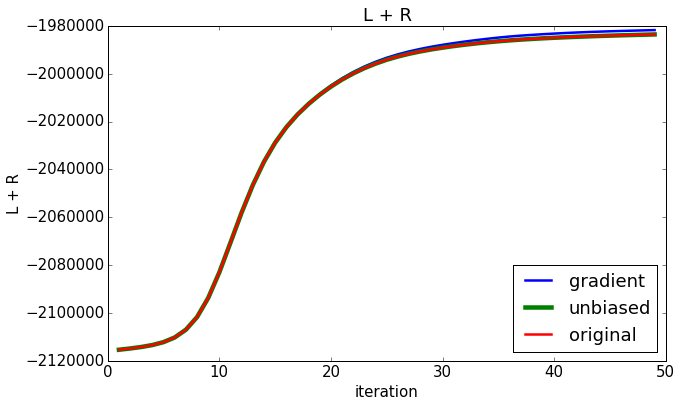
\includegraphics[width=0.31\linewidth]{LR5}
 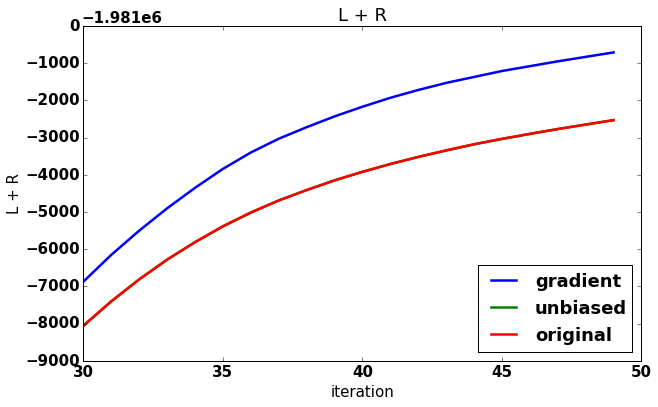
\includegraphics[width=0.31\linewidth]{LR5_tail}
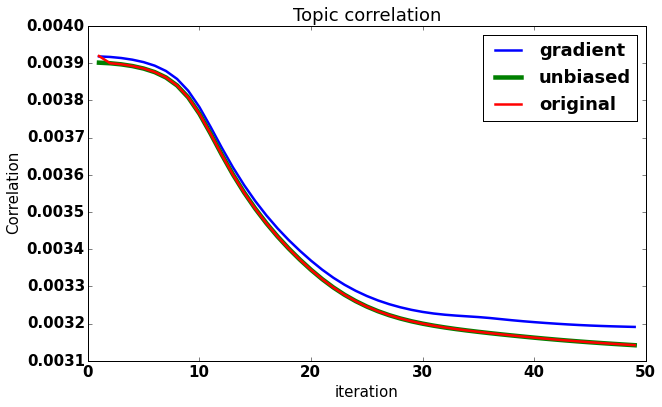
\includegraphics[width=0.31\linewidth]{R5}}\\
 \center{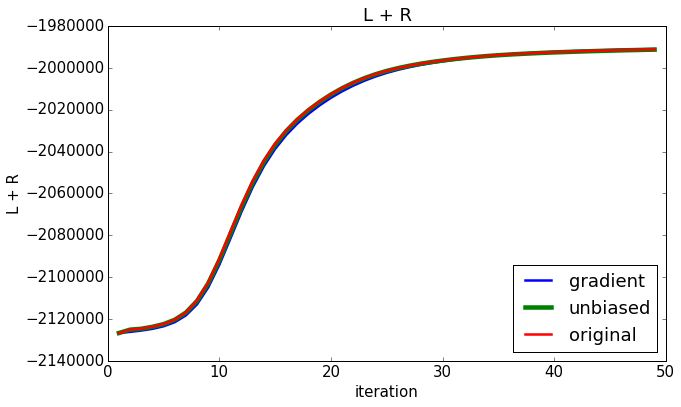
\includegraphics[width=0.31\linewidth]{LR6}
 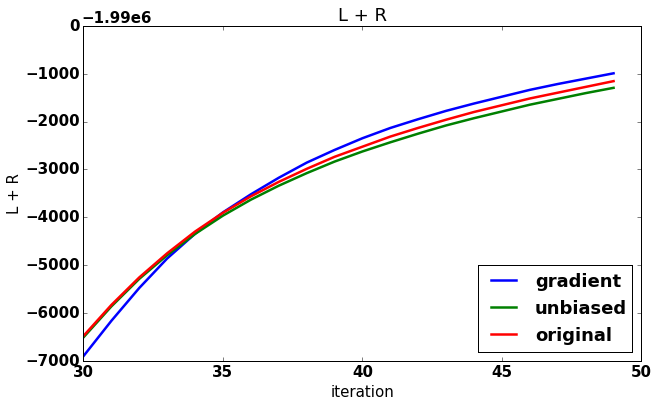
\includegraphics[width=0.31\linewidth]{LR6_tail}
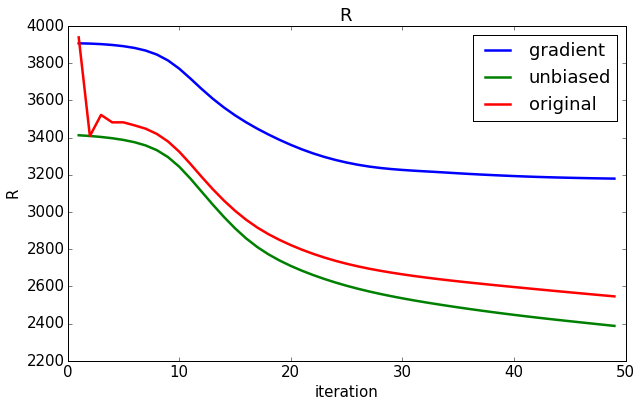
\includegraphics[width=0.31\linewidth]{R6}}\\
}

\headerbox{References}{name=references,column=0,below=pictures,span=3}{
    \textit{Vorontsov K. V., Potapenko A. A.} Additive Regularization of Topic Models // Machine Learning. Special Issue “Data Analysis and Intelligent Optimization with Applications”: Volume 101, Issue 1 (2015), Pp. 303-323.
}

\end{poster}
\end{document}

